\documentclass[11pt,a4paper]{article}

% =================================================================
%  Question Bank -- Unit III: Principles of Numerical Control and Coding
%  Self-contained: all block diagrams / flowcharts drawn with TikZ.
% =================================================================

\usepackage[margin=2cm, headheight=14pt]{geometry}
\usepackage{amsmath}
\usepackage{amssymb}
\usepackage{bm}
\usepackage{array}
\usepackage{booktabs}
\usepackage{enumitem}
\usepackage{xcolor}
\usepackage{tikz}
\usepackage[most]{tcolorbox}
\usepackage{fancyhdr}
\usepackage{helvet}
\renewcommand{\familydefault}{\sfdefault}
\setlength{\emergencystretch}{2em}

\usetikzlibrary{shapes.geometric, arrows.meta, positioning, calc, fit, backgrounds, patterns}

% -------------------------------------------------
% Colour palette (same as the lecture decks)
% -------------------------------------------------
\definecolor{cAccent}{RGB}{0,102,153}
\definecolor{cGreen}{RGB}{34,139,34}
\definecolor{cRed}{RGB}{178,34,34}
\definecolor{cOrange}{RGB}{204,102,0}
\definecolor{cPurple}{RGB}{102,45,145}
\definecolor{cGrayBg}{RGB}{245,246,248}

% -------------------------------------------------
% TikZ styles
% -------------------------------------------------
\tikzset{
	process/.style  ={rectangle, minimum width=2.6cm, minimum height=0.8cm, text centered, align=center, text width=2.6cm, draw=black, fill=blue!8},
	decision/.style ={diamond, aspect=2, minimum width=2.4cm, minimum height=0.9cm, text centered, text width=2.4cm, draw=black, fill=cGreen!18, inner sep=1pt},
	startstop/.style={rectangle, rounded corners=8pt, minimum width=2.2cm, minimum height=0.7cm, text centered, align=center, draw=black, fill=cAccent!25},
	flowarrow/.style={-{Stealth[length=2.5mm]}, thick},
	blk/.style      ={rectangle, draw=black, thick, minimum width=1.9cm, minimum height=0.9cm, align=center, fill=blue!8},
	sumj/.style     ={circle, draw=black, thick, minimum size=0.55cm, inner sep=0pt},
	sig/.style      ={-{Stealth[length=2.2mm]}, thick},
	vflow/.style    ={-{Stealth[length=2mm]}, thick},
}
% valve-symbol helpers
\newcommand{\vspring}[2]{%
	\draw[thick] (#1,#2) -- ++(0.08,0.18) -- ++(0.1,-0.36) -- ++(0.1,0.36) -- ++(0.1,-0.36) -- ++(0.1,0.36) -- ++(0.08,-0.18);}
\newcommand{\vsolenoid}[2]{%
	\draw[thick] ({#1-0.45},{#2-0.22}) rectangle (#1,{#2+0.22});
	\draw[thick] ({#1-0.45},{#2-0.22}) -- (#1,{#2+0.22});}
\newcommand{\vblock}[3]{%
	\draw[thick] (#1,#2) -- (#1,{#2+#3});
	\draw[thick] ({#1-0.12},{#2+#3}) -- ({#1+0.12},{#2+#3});}

% ladder-logic helpers
\newcommand{\ladNO}[3]{%
	\draw[thick] ({#1-0.15},{#2-0.25}) -- ({#1-0.15},{#2+0.25});
	\draw[thick] ({#1+0.15},{#2-0.25}) -- ({#1+0.15},{#2+0.25});
	\node[above=1pt, font=\scriptsize] at (#1,{#2+0.25}) {#3};}
\newcommand{\ladNC}[3]{%
	\ladNO{#1}{#2}{#3}
	\draw[thick] ({#1-0.25},{#2-0.3}) -- ({#1+0.25},{#2+0.3});}
\newcommand{\ladCoil}[3]{%
	\draw[thick] (#1,#2) circle (0.28);
	\node[above=1pt, font=\scriptsize] at (#1,{#2+0.28}) {#3};}

% -------------------------------------------------
% Question / answer layout
% -------------------------------------------------
\newcommand{\opts}[4]{%
	\par\smallskip
	\begin{tabular}{@{}p{0.46\linewidth}p{0.46\linewidth}@{}}
		(a) #1 & (b) #2 \\
		(c) #3 & (d) #4 \\
	\end{tabular}\par}
\newcommand{\ans}[1]{%
	\par\smallskip
	{\color{cGreen!50!black}\textbf{Answer:} #1}\par\medskip}
\newtcolorbox{answer}{breakable, enhanced, colback=cGreen!4, colframe=cGreen!55!black,
	boxrule=0.6pt, arc=2pt, left=6pt, right=6pt, top=4pt, bottom=4pt,
	title={Answer}, fonttitle=\bfseries\small, coltitle=white}
\newcommand{\qmarks}[1]{\hfill\textbf{[#1]}}
\newcommand{\partheading}[2]{%
	\bigskip
	\begin{tcolorbox}[colback=cAccent!10, colframe=cAccent, boxrule=0.6pt, arc=2pt, left=6pt, top=3pt, bottom=3pt]
		\textbf{\large #1} \hfill \textbf{#2}
	\end{tcolorbox}}

\setlist[enumerate,1]{label=\textbf{Q\arabic*.}, leftmargin=*, itemsep=6pt}

\pagestyle{fancy}
\fancyhf{}
\lhead{\small Question Bank --- Unit III}
\rhead{\small Principles of Numerical Control and Coding}
\cfoot{\small \thepage}

\begin{document}

	% -------------------------------------------------
	% Title block
	% -------------------------------------------------
	\begin{center}
		{\Large\bfseries\color{cAccent} Question Bank}\\[4pt]
		{\large\bfseries Unit III: Principles of Numerical Control and Coding}\quad(12 Hrs.)\\[6pt]
		{\small Amit Kumar Singh, Assistant Professor (ECE), School of Naval Architecture and Ocean Engineering\\
			Indian Maritime University, Visakhapatnam Campus}
	\end{center}

	\noindent\textbf{Syllabus:} Basic principles of automation; extending the capabilities of conventional machines through improved devices and manipulators; basic principles of numerical control; CNC, DNC and machining centres; methods of coding and programming; APT programming; adaptive control; economics of numerical control.

	\medskip
	\noindent
	\begin{tabular}{@{}lll@{}}
		\textbf{Part A} & 10 multiple-choice questions & $10\times1 = 10$ marks \\
		\textbf{Part B} & 5 short-answer questions      & $5\times2 = 10$ marks \\
		\textbf{Part C} & 3 long-answer questions       & $3\times10 = 30$ marks \\
	\end{tabular}

	% =================================================================
	\partheading{Part A: Multiple-Choice Questions}{1 mark each}
	% =================================================================
	\begin{enumerate}

		\item In an NC machine tool, the Z axis is always
		\opts{the longest horizontal axis}{a rotary axis}{vertical}{along the spindle axis}
		\ans{(d) Along the spindle axis; $+Z$ moves the tool away from the workpiece.}

		\item The G-code G01 commands
		\opts{rapid positioning}{linear interpolation at feed rate}{circular interpolation CW}{dwell}
		\ans{(b) Linear interpolation (straight-line cutting move) at the programmed feed.}

		\item The M-code M03 means
		\opts{spindle ON, clockwise}{program stop}{coolant ON}{tool change}
		\ans{(a) Spindle ON, clockwise.}

		\item Drilling a pattern of holes needs which type of NC control?
		\opts{Adaptive}{Continuous path}{Point-to-point}{Manual}
		\ans{(c) Point-to-point --- the path between holes does not matter.}

		\item APT stands for
		\opts{Automatic Part Tooling}{Automatically Programmed Tools}{Advanced Programming Technique}{Absolute Position Transfer}
		\ans{(b) Automatically Programmed Tools.}

		\item In DNC, a central computer
		\opts{replaces the machine tool}{is used only for drawing}{controls only one spindle}{stores programs and sends them to many machines}
		\ans{(d) Stores part programs and distributes them to many CNC machines over a network.}

		\item The device that changes tools automatically on a machining centre is called
		\opts{ATC}{APC}{DRO}{MCU}
		\ans{(a) ATC --- Automatic Tool Changer.}

		\item The G-code for absolute programming is
		\opts{G17}{G91}{G90}{G28}
		\ans{(c) G90 (G91 is incremental).}

		\item Adaptive control constraint (ACC) systems keep
		\opts{a process variable such as cutting force at or below a limit}{the spindle speed constant always}{the program unchanged}{the tool cold}
		\ans{(a) A measured variable (force, power, torque) at or below a set limit by adjusting feed/speed.}

		\item The first NC milling machine (1952) was developed at
		\opts{IIT Bombay}{MIT}{Cambridge}{Tokyo University}
		\ans{(b) MIT (with J.\,T.\ Parsons, for the US Air Force).}

	\end{enumerate}

	% =================================================================
	\partheading{Part B: Short-Answer Questions}{2 marks each}
	% =================================================================
	\begin{enumerate}

		\item Define numerical control and name its three basic components. \qmarks{2}
		\begin{answer}
			\textbf{Numerical control (NC)} is a form of programmable automation in which the motions of a machine tool are controlled by a program of coded numbers, letters and symbols. Its three basic components are: (1) the \textbf{part program}, (2) the \textbf{machine control unit (MCU)}, and (3) the \textbf{machine tool} (processing equipment).
		\end{answer}

		\item Distinguish between absolute and incremental positioning with an example. \qmarks{2}
		\begin{answer}
			In \textbf{absolute} positioning (G90) every coordinate is measured from the program zero; in \textbf{incremental} positioning (G91) each move is measured from the previous position.\\
			Example: moving from A(10, 10) to B(40, 10): absolute \texttt{X40 Y10}; incremental \texttt{X30 Y0}.
		\end{answer}

		\item An open-loop NC axis uses a stepper motor of 200 steps/rev directly coupled to a lead screw of 5 mm pitch. Find the BLU and the pulses needed for a 100 mm move. \qmarks{2}
		\begin{answer}
			$\text{BLU} = \dfrac{p}{n_s} = \dfrac{5}{200} = \mathbf{0.025\ mm}$.\qquad Pulses $= \dfrac{100}{0.025} = \mathbf{4000}$.
		\end{answer}

		\item Explain the word-address block format with an example. \qmarks{2}
		\begin{answer}
			In the word-address format every word begins with a \textbf{letter address} that tells the controller the meaning of the number that follows; words may be in any order and only changed words need be written.\\
			Example: \texttt{N050 G01 X25.0 Y30.0 F200 S1000 M03} --- block 50, linear feed to (25, 30) at 200 mm/min, spindle 1000 rpm clockwise.
		\end{answer}

		\item A CNC machine costs Rs 40 lakh and gives net savings of Rs 10 lakh per year. Find the payback period and state its meaning. \qmarks{2}
		\begin{answer}
			Payback $= \dfrac{\text{investment}}{\text{net annual saving}} = \dfrac{40}{10} = \mathbf{4\ years}$. It is the time needed for the savings to recover the initial investment; a shorter payback means a more attractive investment.
		\end{answer}

	\end{enumerate}

	% =================================================================
	\partheading{Part C: Long-Answer Questions}{10 marks each}
	% =================================================================
	\begin{enumerate}

		% -------------------------------------------------------------
		\item With neat block diagrams, explain open-loop and closed-loop NC systems. Explain the basic components of a CNC system and list the advantages of CNC over conventional NC. \qmarks{10}
		\begin{answer}
			\textbf{(a) Open-loop NC system}
			\begin{center}
				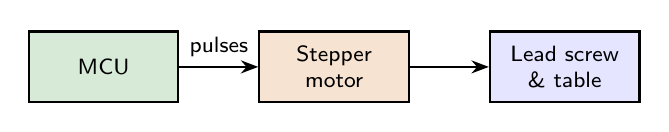
\begin{tikzpicture}[font=\footnotesize, node distance=1.0cm]
					\node[blk, fill=cGreen!18] (c) {MCU};
					\node[blk, right=of c, fill=cOrange!18] (m) {Stepper\\ motor};
					\node[blk, right=of m, fill=blue!10] (s) {Lead screw\\ \& table};
					\draw[sig] (c) -- node[above] {pulses} (m); \draw[sig] (m) -- (s);
				\end{tikzpicture}
			\end{center}
			The MCU sends a counted number of pulses to a stepper motor; each pulse moves the table one BLU. There is \textbf{no feedback}, so missed steps (overload) are not detected. It is simple and cheap and is used for light-duty machines.

			\textbf{(b) Closed-loop NC system}
			\begin{center}
				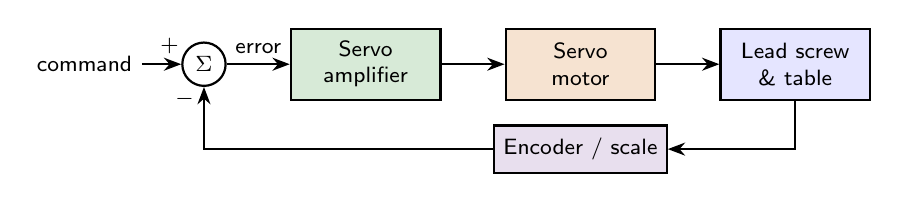
\begin{tikzpicture}[font=\footnotesize, node distance=0.8cm]
					\node (r) {command};
					\node[sumj, right=0.5cm of r] (s) {$\Sigma$};
					\node[blk, right=of s, fill=cGreen!18] (c) {Servo\\ amplifier};
					\node[blk, right=of c, fill=cOrange!18] (m) {Servo\\ motor};
					\node[blk, right=of m, fill=blue!10] (t) {Lead screw\\ \& table};
					\node[blk, below=0.3cm of m, fill=cPurple!15, minimum height=0.6cm] (e) {Encoder / scale};
					\draw[sig] (r) -- node[above, pos=0.7] {$+$} (s);
					\draw[sig] (s) -- node[above] {error} (c);
					\draw[sig] (c) -- (m); \draw[sig] (m) -- (t);
					\draw[sig] (t.south) |- (e);
					\draw[sig] (e) -| node[left, pos=0.9] {$-$} (s);
				\end{tikzpicture}
			\end{center}
			A servo motor drives the table; an \textbf{encoder or linear scale} measures the actual position and feeds it back. The MCU compares it with the command and corrects the error, giving high accuracy even under varying loads.

			\textbf{(c) Components of a CNC system}
			\begin{itemize}[itemsep=1pt]
				\item \textbf{Program input} --- keyboard (MDI), USB, network/DNC.
				\item \textbf{CPU and memory} --- store the program, decode blocks, perform \textbf{interpolation} and compensation.
				\item \textbf{Servo drives} --- one per axis plus the spindle drive.
				\item \textbf{PLC section} --- handles M-codes: spindle, coolant, tool changer, door interlocks.
				\item \textbf{Feedback devices} --- encoders, tachometers, linear scales.
				\item \textbf{Operator panel / display} --- graphics, diagnostics.
			\end{itemize}

			\textbf{(d) Advantages of CNC over hard-wired NC}: program stored and edited at the machine; any interpolation in software; tool-length and cutter-radius compensation; canned cycles and sub-programs; graphic simulation; diagnostics; easy DNC networking; one program runs many parts without re-reading tape.
		\end{answer}

		% -------------------------------------------------------------
		\item Explain the steps of manual part programming with a flowchart. Write a word-address (G-code) part program to mill the outer profile shown, using a 10 mm end mill, depth 2 mm, spindle 1200 rpm and feed 200 mm/min. \qmarks{10}
		\begin{center}
			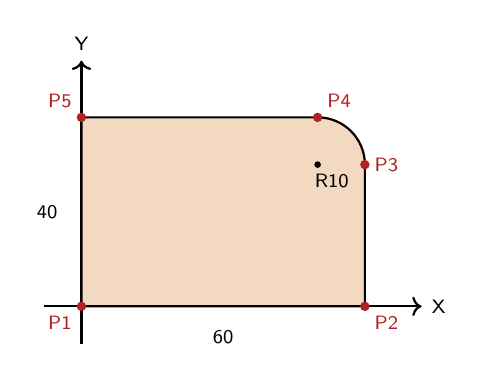
\begin{tikzpicture}[font=\scriptsize, scale=0.06]
				\draw[->, thick] (-8,0) -- (72,0) node[right] {X};
				\draw[->, thick] (0,-8) -- (0,52) node[above] {Y};
				\filldraw[fill=cOrange!25, draw=black, thick] (0,0) -- (60,0) -- (60,30) arc (0:90:10) -- (0,40) -- cycle;
				\foreach \p/\n/\pos in {(0,0)/P1/below left, (60,0)/P2/below right, (60,30)/P3/right, (50,40)/P4/above right, (0,40)/P5/above left}
				\fill[cRed] \p circle (1.0) node[\pos] {\n};
				\fill (50,30) circle (0.7);
				\node[below] at (53,30) {R10};
				\node[below] at (30,-3) {60};
				\node[left] at (-3,20) {40};
			\end{tikzpicture}
		\end{center}
		\begin{answer}
			\noindent\begin{minipage}[t]{0.42\linewidth}
				\textbf{(a) Steps in manual part programming}
				\begin{center}
					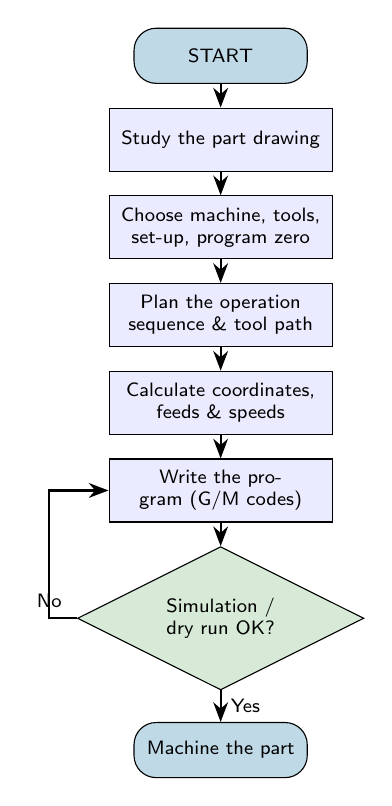
\begin{tikzpicture}[font=\scriptsize, node distance=0.3cm]
						\node[startstop] (st) {START};
						\node[process, below=of st] (a) {Study the part drawing};
						\node[process, below=of a] (b) {Choose machine, tools, set-up, program zero};
						\node[process, below=of b] (c) {Plan the operation sequence \& tool path};
						\node[process, below=of c] (d) {Calculate coordinates, feeds \& speeds};
						\node[process, below=of d] (e) {Write the program (G/M codes)};
						\node[decision, below=of e] (f) {Simulation / dry run OK?};
						\node[startstop, below=0.4cm of f] (g) {Machine the part};
						\draw[flowarrow] (st) -- (a); \draw[flowarrow] (a) -- (b); \draw[flowarrow] (b) -- (c);
						\draw[flowarrow] (c) -- (d); \draw[flowarrow] (d) -- (e); \draw[flowarrow] (e) -- (f);
						\draw[flowarrow] (f) -- node[right] {Yes} (g);
						\draw[flowarrow] (f.west) -- ++(-0.35,0) node[above] {No} |- (e.west);
					\end{tikzpicture}
				\end{center}
			\end{minipage}\hfill
			\begin{minipage}[t]{0.55\linewidth}
				\textbf{(b) Part program} (program zero at P1, top face Z0; tool centre on the outline for simplicity)
				\begin{center}
					\footnotesize
					\setlength{\tabcolsep}{3pt}
					\begin{tabular}{@{}>{\ttfamily}l>{\scriptsize}l@{}}
						\toprule
						\textrm{\textbf{Block}} & \textbf{Meaning} \\
						\midrule
						O1001                 & program number \\
						N10 G21 G90 G17       & metric, absolute, XY plane \\
						N20 T01 M06           & load tool 1 (10 mm end mill) \\
						N30 G00 X0 Y0 Z5.0    & rapid above P1 \\
						N40 S1200 M03 M08     & spindle CW, coolant ON \\
						N50 G01 Z-2.0 F100    & plunge 2 mm \\
						N60 X60.0 F200        & P1 $\rightarrow$ P2 \\
						N70 Y30.0             & P2 $\rightarrow$ P3 \\
						N80 G03 X50.0 Y40.0 R10.0 & arc P3 $\rightarrow$ P4 (CCW) \\
						N90 G01 X0            & P4 $\rightarrow$ P5 \\
						N100 Y0               & P5 $\rightarrow$ P1 \\
						N110 G00 Z50.0 M09    & retract, coolant OFF \\
						N120 M05              & spindle stop \\
						N130 M30              & end, rewind \\
						\bottomrule
					\end{tabular}
				\end{center}
			\end{minipage}

			\medskip
			\textbf{Notes:} G01/G00 and X/Y words are \textbf{modal} --- they stay active until changed, so repeated codes are omitted. The arc from P3 to P4 is counter-clockwise about the centre (50, 30), hence G03. To cut the true outline with the tool outside the part, cutter-radius compensation \texttt{G41/G42} with an offset of 5 mm would be added.
		\end{answer}

		% -------------------------------------------------------------
		\item Explain APT programming: the structure of an APT system (with a block diagram), the four types of APT statements, and the motion statements. Write the APT motion statements for contouring the part of Q2. \qmarks{10}
		\begin{answer}
			\textbf{(a) APT system}
			\begin{center}
				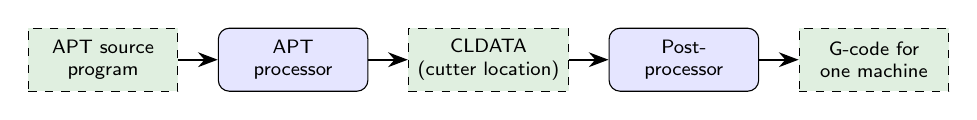
\begin{tikzpicture}[every node/.style={font=\scriptsize}, node distance=0.5cm,
					tool/.style={rectangle, draw=black, rounded corners, minimum width=1.9cm, minimum height=0.8cm, align=center, fill=blue!10},
					art/.style ={rectangle, draw=black, dashed, minimum width=1.9cm, minimum height=0.8cm, align=center, fill=cGreen!14}]
					\node[art] (src) {APT source\\ program};
					\node[tool, right=of src] (proc) {APT\\ processor};
					\node[art, right=of proc] (cl) {CLDATA\\ (cutter location)};
					\node[tool, right=of cl] (post) {Post-\\ processor};
					\node[art, right=of post] (gc) {G-code for\\ one machine};
					\draw[flowarrow] (src) -- (proc); \draw[flowarrow] (proc) -- (cl);
					\draw[flowarrow] (cl) -- (post); \draw[flowarrow] (post) -- (gc);
				\end{tikzpicture}
			\end{center}
			APT (Automatically Programmed Tools, MIT 1956--59) lets the programmer describe the \textbf{geometry} and \textbf{tool motion} in English-like statements. The \textbf{processor} computes the cutter-centre path (CLDATA), independent of the machine. The \textbf{post-processor} converts CLDATA into the codes of a particular machine/controller.

			\textbf{(b) Four types of statements}
			\begin{center}
				\small
				\begin{tabular}{@{}p{3.0cm}p{4.2cm}p{6.4cm}@{}}
					\toprule
					\textbf{Type} & \textbf{Purpose} & \textbf{Example} \\
					\midrule
					Geometry       & define points, lines, circles, planes & \texttt{P1 = POINT/0, 0, 0}; \texttt{L1 = LINE/P1, P2} \\
					Motion         & describe the tool path                & \texttt{FROM/P0}; \texttt{GORGT/L1, PAST, L2} \\
					Post-processor & speeds, feeds, coolant                & \texttt{SPINDL/1200, CLW}; \texttt{FEDRAT/200} \\
					Auxiliary      & part name, cutter, tolerance, end     & \texttt{PARTNO}; \texttt{CUTTER/10}; \texttt{FINI} \\
					\bottomrule
				\end{tabular}
			\end{center}

			\textbf{(c) Motion statements}: point-to-point \texttt{FROM/}, \texttt{GOTO/}, \texttt{GODLTA/}; contouring direction words \texttt{GOLFT}, \texttt{GORGT}, \texttt{GOFWD}, \texttt{GOBACK}, \texttt{GOUP}, \texttt{GODOWN}; check-surface modifiers \texttt{TO}, \texttt{ON}, \texttt{PAST}, \texttt{TANTO}; tool side \texttt{TLLFT}, \texttt{TLRGT}, \texttt{TLON}.

			\textbf{(d) APT program for the part of Q2} (L1: $y=0$, L2: $x=60$, C1: centre (50, 30) R10, L3: $y=40$, L4: $x=0$, PL1: $z=-2$, start point P0 $(-20,-20,10)$)
			\begin{center}
				\small
				\begin{tabular}{@{}>{\ttfamily}l>{\footnotesize}l@{}}
					\toprule
					\textrm{\textbf{Statement}} & \textbf{Meaning} \\
					\midrule
					CUTTER/10.0                  & 10 mm cutter \\
					SPINDL/1200, CLW \quad FEDRAT/200 & spindle and feed \\
					FROM/P0                      & start point \\
					GO/TO, L1, TO, PL1, TO, L4   & go down to touch L1 and L4 at depth PL1 \\
					TLRGT, GORGT/L1, PAST, L2    & tool right of L1, cut to beyond L2 \\
					GOLFT/L2, TANTO, C1          & turn left along L2 up to tangent with C1 \\
					GOFWD/C1, TANTO, L3          & follow the arc to tangent with L3 \\
					GOFWD/L3, PAST, L4           & along L3 to beyond L4 \\
					GOLFT/L4, PAST, L1           & down L4 to beyond L1 \\
					GOTO/P0 \quad FINI           & return, end \\
					\bottomrule
				\end{tabular}
			\end{center}
		\end{answer}

	\end{enumerate}

\end{document}
